\subsection{Nebelkammer}

Entwickelt wurde die Nebelkammer von Charles Wilson (1869-1959). Ausgangspunkt ist die
Van-der-Waals-Gleichung. Unter bestimmten Bedingungen ist es möglich, übersättigten Dampf oder
übersättigte Flüssigkeit herzustellen.

\begin{figure}[H]
	\centering
	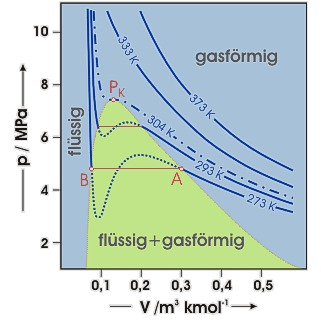
\includegraphics[width=0.5\textwidth]{Fig-02-01.jpg}
	\caption{PV-Isothermen eines realen Gases (CO$_2$) - Druck gegen Gas für konstante Temperaturen}
\end{figure}

Beim Herstellen einer Übersättigung durch langsames Abkühlen nutzt man aus, dass warme Gase
größere Sättigungswerte haben als kalte. Die Idee hinter der Nebelkammer ist es, übersättigten Dampf
zu erzeugen und durch einfliegende Teilchen erzeugte ionisierte Gasatome als Kondensationskeime für
Dampf zu erhalten: es entsteht eine Nebelspur.
\\
Eine technische Realisation war die Expansionsnebelkammer von Alexander Langsdorf 1936. In dieser
entsteht eine übersättigte Schicht durch eine schnelle Volumenvergrößerung (adiabatische Expansion).
Die maximale Beobachtungszeit liegt allerdings nur bei $10-100\,$ms.

\begin{figure}[H]
	\centering
	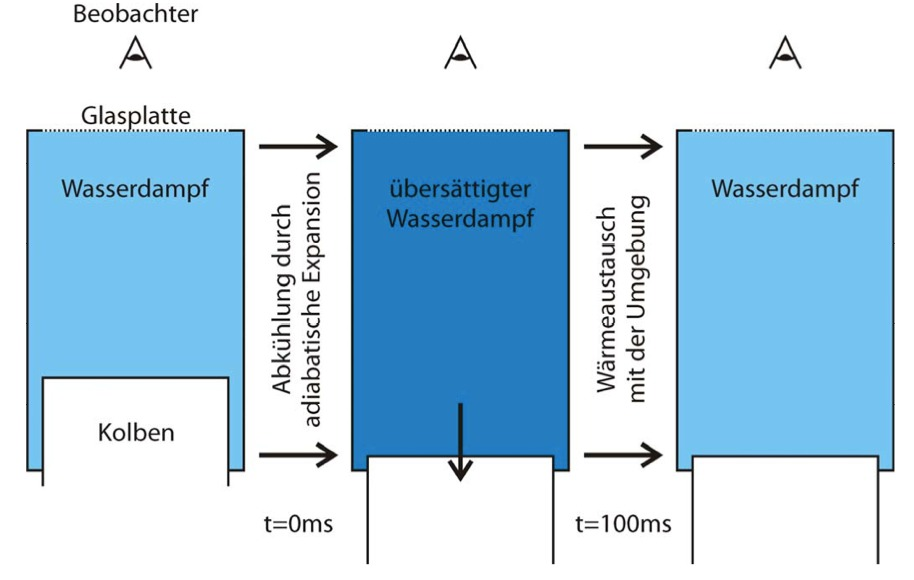
\includegraphics[width=0.75\textwidth]{Fig-02-02.jpg}
\end{figure}

In der Diffusionsnebelkammer dagegen wird die übersättigte Schicht ständig aufrecht erhalten. Die
Idee ist, den unteren Teil zu kühlen ($-10-20^\circ$C) und den oberen Teil zu heizen (ca.
$40^\circ$C). Somit diffundiert der entstandene Dampf nach unten und wird auf dem Weg unter seinen
Taupunkt abgekühlt, wobei die übersättigte Schicht im unteren Bereich der Kammer entsteht. 
\\
Entdeckungen durch die Nebelkammer:

\begin{itemize}
  \item 1932 Positron (Carl Anderson)
  \item 1936 Myon (Carl Anderson)
  \item 1947 Kaon
\end{itemize}

\subsection{Blasenkammer}

Die Blasenkammer beruht auf einem ähnlichen Prinzip wie die Nebelkammer. Wir bringen einen mit
Flüssigkeit kurz unterhalb des Siedepunktes (Wasserstoff, Xenon, \ldots) gefüllten Zylinder unter
hohem Druck ($5-20\,$atm) in ein homogenes Magnetfeld. Kurz vor dem Teilcheneinschuss wird der Druck
stark verringert, sodass sich die Temperatur der Flüssigkeit oberhalb des Siedepunktes befindet.
Einlaufende Teilchen ionisieren nun Atome, welche als Keime für Gasblasen diesen.
\\
$10\,$ms nach dem Teilcheinschuss werden mit mehreren Kameras von unterschiedlichen Positionen aus
Fotos mit Blitzlicht geschossen, was eine 3D-Rekonstruktion ermöglicht. Nachfolgend wird der Druck
wieder erhöht.
Ein solcher Zyklus dauert $\frac{1}{10}\,$s. 
\\
Entwickelt wurde dieser Aufbau von Glaser (1950).

\begin{figure}[htbp]
	\begin{minipage}[b]{0.5\textwidth}
		\begin{figure}[H]
		\centering
		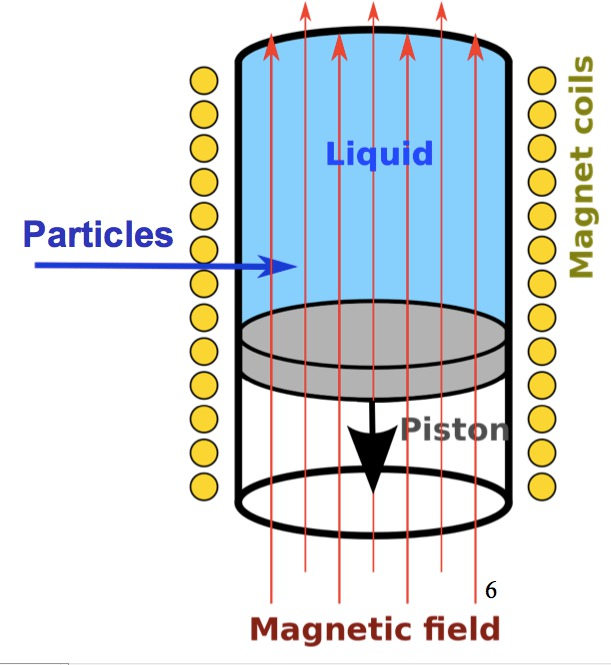
\includegraphics[width=\textwidth]{Fig-02-04.jpg}
		\end{figure}
	\end{minipage}
	\hfill
	\begin{minipage}[b]{0.5\textwidth}
		\begin{figure}[H]
		\centering
		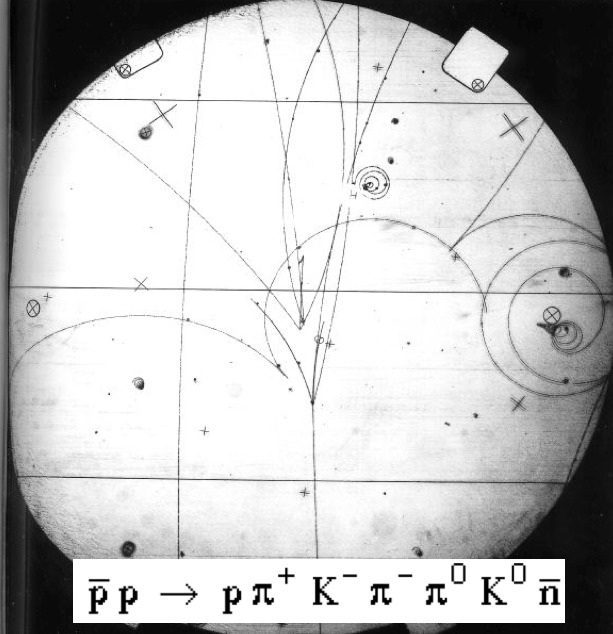
\includegraphics[width=\textwidth]{Fig-02-05.jpg}
		\end{figure}
	\end{minipage}
\end{figure}

Vorteile gegenüber der Nebelkammer:

\begin{itemize}
  \item 3D-Rekonstruktion
  \item große Kammer: viel Targetmaterial, genaue Impulsmessung
\end{itemize}

Nachteile gegenüber der Nebelkammer:

\begin{itemize}
  \item geringe Wiederholungsrate
  \item schwierige Datenanalyse
  \item nicht verwendbar für "`colliding beams"'
\end{itemize}

Eine wichtige Entdeckung waren neutrale Ströme 1973 mit Gargamelle. 

\subsection*{Zusammenfassung}

Nebel- und Blasenkammer sind Konstruktionen, bei denen der Detektor gleichzeitig das Target ist.
Beide sind heute vollkommen ungeeignet, da die Auswertung der Fotos zu langwierig und ungenau sind.
Es werden Detektoren mit elektronischer Auslese benötigt.
